\chapter{Gretl and R}
\label{chap:gretlR}

\section{Introduction}
\label{R-intro}

\app{R} is, by far, the largest free statistical
project.\footnote{\app{R}'s homepage is at
  \url{http://www.r-project.org/}.} Like gretl, it is a GNU project
and the two have a lot in common; however, gretl's approach focuses on
ease of use much more than \app{R}, which instead aims to encompass
the widest possible range of statistical procedures.

As is natural in the free software ecosystem, we don't view ourselves
as competitors to \app{R},\footnote{OK, who are we kidding? But it's
  \emph{friendly} competition!} but rather as projects sharing a
common goal who should support each other whenever possible. For this
reason, gretl provides a way to interact with \app{R} and thus enable
users to pool the capabilities of the two packages.

In this chapter, we will explain how to exploit \app{R}'s power from
within gretl. We assume that the reader has a working installation of
\app{R} available and a basic grasp of \app{R}'s syntax.\footnote{The
  main reference for \app{R} documentation is
  \url{http://cran.r-project.org/manuals.html}.  In addition, \app{R}
  tutorials abound on the Net; as always, Google is your friend.}

Despite several valiant attempts, no graphical shell has gained wide
acceptance in the \app{R} community: by and large, the standard method
of working with \app{R} is by writing scripts, or by typing commands
at the \app{R} prompt, much in the same way as one would write
gretl scripts or work with the gretl console. In this
chapter, the focus will be on the methods available to execute \app{R}
commands without leaving gretl.

\section{Starting an interactive \app{R} session}
\label{sec:R-interactive}

The easiest way to use \app{R} from gretl is in interactive
mode.  Once you have your data loaded in gretl, you can select
the menu item ``Tools, Start GNU R'' and an interactive \app{R}
session will be started, with your dataset automatically pre-loaded.

\subsection{A simple example: OLS on cross-section data}
\label{sec:R-ols-ex}

For this example we use Ramanathan's dataset \texttt{data4-1}, one of
the sample files supplied with gretl.  We first run, in
gretl, an OLS regression of \texttt{price} on \texttt{sqft},
\texttt{bedrms} and \texttt{baths}.  The basic results are shown in
Table \ref{tab:data4-1-gretlOLS}.

\begin{table}[htbp]
\caption{OLS house price regression via gretl}
\label{tab:data4-1-gretlOLS}
\begin{center}

\begin{tabular*}{0.75\textwidth}{@{\extracolsep{\fill}}
l% col 1: varname
  D{.}{.}{-1}% col 2: coeff
    D{.}{.}{-1}% col 3: sderr
      D{.}{.}{-1}% col 4: t-stat
        D{.}{.}{4}}% col 5: p-value (or slope)
Variable &
  \multicolumn{1}{c}{Coefficient} &
    \multicolumn{1}{c}{Std.\ Error} &
      \multicolumn{1}{c}{$t$-statistic} &
        \multicolumn{1}{c}{p-value} \\[1ex]
const &
  129.062 &
    88.3033 &
      1.4616 &
        0.1746 \\
sqft &
  0.154800 &
    0.0319404 &
      4.8465 &
        0.0007 \\
bedrms &
  -21.587 &
    27.0293 &
      -0.7987 &
        0.4430 \\
baths &
  -12.192 &
    43.2500 &
      -0.2819 &
        0.7838 \\
\end{tabular*}
\end{center}
\end{table}

We will now replicate the above results using \app{R}. Select 
the menu item ``Tools, Start GNU R''. A window similar to the one
shown in figure \ref{fig:Rwind1} should appear.

\begin{figure}[htbp]
  \centering
  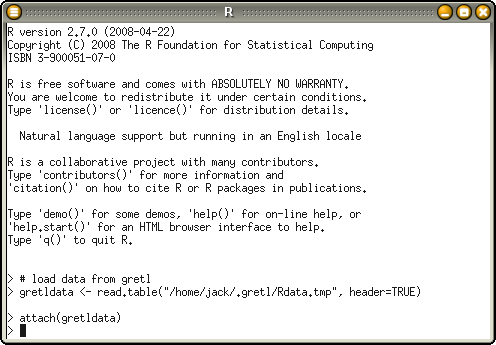
\includegraphics[scale=0.7]{figures/Rwindow-1}
  \caption{\app{R} window}
  \label{fig:Rwind1}
\end{figure}

The actual look of the \app{R} window may be somewhat different from
what you see in Figure~\ref{fig:Rwind1} (especially for Windows
users), but this is immaterial. The important point is that you have a
window where you can type commands to \app{R}. If the above procedure
doesn't work and no \app{R} window opens, it means that gretl
was unable to launch \app{R}.  You should ensure that \app{R} is
installed and working on your system and that gretl knows where
it is. The relevant settings can be found by selecting the ``Tools,
Preferences, General'' menu entry, under the ``Programs'' tab.

Assuming \app{R} was launched successfully, you will see notification
that the data from gretl are available.  In the background,
gretl has arranged for two \app{R} commands to be executed, one
to load the gretl dataset in the form of a \emph{data frame}
(one of several forms in which \app{R} can store data) and one to
\emph{attach} the data so that the variable names defined in the
gretl workspace are available as valid identifiers within
\app{R}.

In order to replicate gretl's OLS estimation, go into the \app{R}
window and type at the prompt
\begin{code}
  model <- lm(price ~ sqft + bedrms + baths)
  summary(model)
\end{code}

\begin{figure}[htbp]
  \centering
  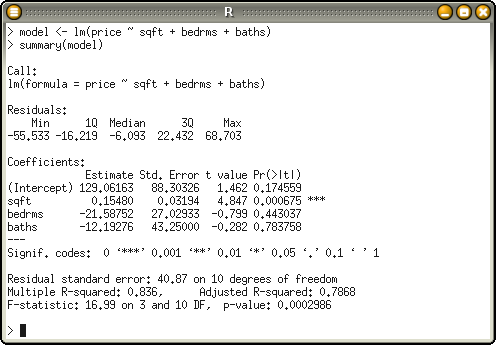
\includegraphics[scale=0.7]{figures/Rwindow-2}
  \caption{OLS regression on house prices via \app{R}}
  \label{fig:Rwind2}
\end{figure}

You should see something similar to
Figure~\ref{fig:Rwind2}. Surprise---the estimates coincide! To get
out, just close the \app{R} window or type \verb|q()| at the \app{R}
prompt.

\subsection{Time series data}
\label{sec:R-ols-arma}

We now turn to an example which uses time series data: we
will compare gretl's and \app{R}'s estimates of Box and Jenkins'
immortal ``airline'' model. The data are contained in the \texttt{bjg}
sample dataset. The following gretl code
\begin{code}
open bjg
arima 0 1 1 ; 0 1 1 ; lg --nc
\end{code}
produces the estimates shown in Table \ref{tab:airline-gretl}.

\begin{table}[htbp]
\caption{Airline model from Box and Jenkins (1976) -- selected
  portion of gretl's estimates}
\label{tab:airline-gretl}
\begin{center}

\begin{tabular*}{0.75\textwidth}{@{\extracolsep{\fill}}
l% col 1: varname
  D{.}{.}{-1}% col 2: coeff
    D{.}{.}{-1}% col 3: sderr
      D{.}{.}{-1}% col 4: t-stat
        D{.}{.}{4}}% col 5: p-value (or slope)
Variable &
  \multicolumn{1}{c}{Coefficient} &
    \multicolumn{1}{c}{Std.\ Error} &
      \multicolumn{1}{c}{$t$-statistic} &
        \multicolumn{1}{c}{p-value} \\[1ex]
$\theta_{1}$ &
  -0.401824 &
    0.0896421 &
      -4.4825 &
        0.0000 \\
$\Theta_{1}$ &
  -0.556936 &
    0.0731044 &
      -7.6184 &
        0.0000 \\
\end{tabular*}

\begin{tabular}{lD{.}{.}{-1}}
Variance of innovations & 0.00134810 \\
Log-likelihood & 244.696 \\
Akaike information criterion & -483.39 
\end{tabular}
\end{center}
\end{table}

If we now open an \app{R} session as described in the previous
subsection, the data-passing mechanism is slightly different.  Since
our data were defined in gretl as time series, we use an \app{R}
\emph{time-series} object (\emph{ts} for short) for the transfer.  In
this way we can retain in \app{R} useful information such as the
periodicity of the data and the sample limits.  The downside is that
the names of individual series, as defined in gretl, are not
valid identifiers. In order to extract the variable \texttt{lg}, one
needs to use the syntax \verb|lg <- gretldata[, "lg"]|.

ARIMA estimation can be carried out by issuing the following two
\app{R} commands:
\begin{code}
lg <- gretldata[, "lg"]
arima(lg, c(0,1,1), seasonal=c(0,1,1))
\end{code}

which yield

\begin{code}
Coefficients:
          ma1     sma1
      -0.4018  -0.5569
s.e.   0.0896   0.0731

sigma^2 estimated as 0.001348:  log likelihood = 244.7,  aic = -483.4
\end{code}

Happily, the estimates again coincide.

\section{Running an \app{R} script}
\label{sec:R-scripts}

Opening an \app{R} window and keying in commands is a convenient
method when the job is small. In some cases, however, it would be
preferable to have \app{R} execute a script prepared in advance. 
One way to do this is via the \texttt{source()} command in
\app{R}.  Alternatively, gretl offers the facility to edit an
\app{R} script and run it, having the current dataset pre-loaded
automatically. This feature can be accessed via the ``File, Script
Files'' menu entry.  By selecting ``User file'', one can load a
pre-existing \app{R} script; if you want to create a new script
instead, select the ``New script, R script'' menu entry.

\begin{figure}[htbp]
  \centering
  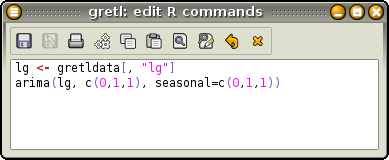
\includegraphics[scale=0.7]{figures/R-edit1}
  \caption{Editing window for \app{R} scripts}
  \label{fig:R-edit1}
\end{figure}
In either case, you are presented with a window very similar to
the editor window used for ordinary gretl scripts, as in
Figure~\ref{fig:R-edit1}.

There are two main differences.  First, you get syntax highlighting for
\app{R}'s syntax instead of gretl's. Second, clicking on the
Execute button (the gears icon), launches an instance of \app{R} in
which your commands are executed.  Before \app{R} is actually run, you
are asked if you want to run \app{R} interactively or not (see
Figure~\ref{fig:R-exec-mode}).

\begin{figure}[htbp]
  \centering
  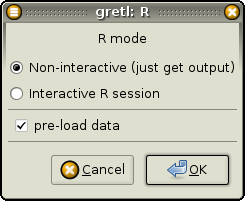
\includegraphics[scale=0.7]{figures/R-exec-mode}
  \caption{Editing window for \app{R} scripts}
  \label{fig:R-exec-mode}
\end{figure}

An interactive run opens an \app{R} instance similar to the one seen
in the previous section: your data will be pre-loaded (if the
``pre-load data'' box is checked) and your commands will
be executed. Once this is done, you will find yourself at the \app{R}
prompt, where you can enter more commands.

A non-interactive run, on the other hand, will execute your script,
collect the output from \app{R} and present it to you in an output
window; \app{R} will be run in the background. If, for example, the
script in Figure~\ref{fig:R-edit1} is run non-interactively, a window
similar to Figure~\ref{fig:R-output1} will appear.

\begin{figure}[htbp]
  \centering
  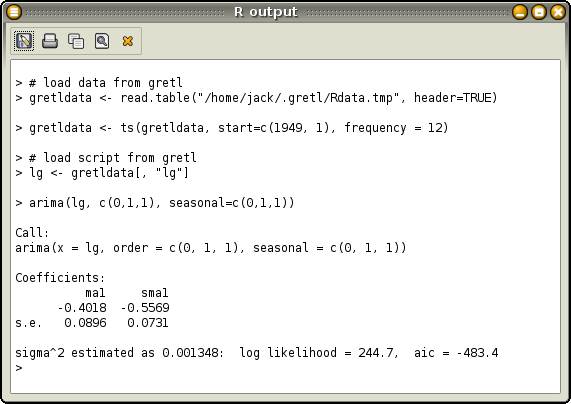
\includegraphics[scale=0.7]{figures/R-output1}
  \caption{Output from a non-interactive \app{R} run}
  \label{fig:R-output1}
\end{figure}

\section{Taking stuff back and forth}
\label{sec:R-passing-data}

As regards the passing of data between the two programs, so far we
have only considered passing series from gretl to \app{R}. In
order to achieve a satisfactory degree of interoperability, more is
needed.  In the following sub-sections we see how matrices can be
exchanged, and how data can be passed from \app{R} back to
gretl.

\subsection{Passing matrices from gretl to \app{R}}

For passing matrices from gretl to \app{R}, you can use the
\texttt{mwrite} matrix function described in section
\ref{sec:matrix-csv}. For example, the following gretl code
fragment generates the matrix 
\[ 
A = \left[
  \begin{array}{ccc}
    3 &  7 &  11 \\ 
    4 &  8 &  12 \\ 
    5 &  9 &  13 \\ 
    6 & 10 &  14 
  \end{array}
\right]
\] 
and stores it into the file \texttt{mymatfile.mat} in the user's
``dotdir''(see section~\ref{sec:named-strings}). Note that writing to
this special directory, which is sure to exist and be writable by the
user, is mandated by the non-zero value for the third, optional
argument to \texttt{mwrite}.
\begin{code}
  matrix A = mshape(seq(3,14),4,3)
  err = mwrite(A, "mymatfile.mat", 1)
\end{code}
The recommended \app{R} code to import such a matrix is
\begin{code}
  A <- gretl.loadmat("mymatfile.mat")
\end{code}

The function \texttt{gretl.loadmat}, which is predefined when \app{R}
is called from gretl, retrieves the matrix from dotdir.  (The
``\texttt{.mat}'' extension for gretl matrix files is not compulsory;
you can name these files as you wish.)

It's also possible to take more control over the details of the
transer if you wish. You have the built-in string variable
\verb|$dotdir| in gretl, while in \app{R} you have the same variable
under the name \texttt{gretl.dotdir}. To use a location other than
\verb|$dotdir| you may (a) omit the third argument to \texttt{mwrite}
and supply a full path to the matrix file, and (b) use a more generic
approach to reading the file in \app{R}. Here's an example:

Gretl side:
\begin{code}
  mwrite(A, "/path/to/mymatfile.mat")
\end{code}
\app{R} side:
\begin{code}
  A <- as.matrix(read.table("/path/to/mymatfile.mat", skip=1))
\end{code}

\subsection{Passing data from \app{R} to gretl}
\label{sec:Rpassing-data}

For passing data in the opposite direction, gretl defines a special
function that can be used in the \app{R} environment. An \app{R}
object will be written as a temporary file in
\verb|$dotdir|, from where it can be easily retrieved from within
gretl.

The name of this function is \texttt{gretl.export()}; it takes one
required argument, the object to be exported. At present, the objects
that can be exported with this method are matrices, data frames and
time-series objects. The function creates a text file, by default with
the same name as the exported object (plus an appropriate suffix),
in gretl's temporary directory. Data frames and time-series objects
are stored as CSV files, and can be retrieved by using gretl's
\texttt{append} command.  Matrices are stored in a special text format
that is understood by gretl (see section~\ref{sec:matrix-csv}); the
file suffix is in this case \texttt{.mat}, and to read the matrix in
gretl you must use the \texttt{mread()} function.

This function also has an optional second argument, namely a string
which specifies a basename for the export file, in case you want to
use a name other than that attached to the object within \app{R}. As
in the default case an appropriate suffix, \texttt{.csv} or
\texttt{.mat}, will be added to the basename.

As an example, we take the airline data and use them to estimate a
structural time series model \`a la \cite{harvey89}.\footnote{The
  function package \package{StucTiSM} is available to handle this
  class of models natively in \app{gretl}.} The model we will use is
the \emph{Basic Structural Model} (BSM), in which a time series is
decomposed into three terms:
\[
  y_t = \mu_t + \gamma_t + \varepsilon_t
\]
where $\mu_t$ is a trend component, $\gamma_t$ is a seasonal component
and $\varepsilon_t$ is a noise term. In turn, the following is assumed
to hold:
\begin{eqnarray*}
  \Delta \mu_t & = & \beta_{t-1} + \eta_t \\
  \Delta \beta_t & = & \zeta_t \\
  \Delta_s \gamma_t & = & \Delta \omega_t
\end{eqnarray*}
where $\Delta_s$ is the seasonal differencing operator, $(1-L^s)$, and
$\eta_t$, $\zeta_t$ and $\omega_t$ are mutually uncorrelated white
noise processes. The object of the analysis is to estimate the
variances of the noise components (which may be zero) and to recover
estimates of the latent processes $\mu_t$ (the ``level''), $\beta_t$
(the ``slope'') and $\gamma_t$.

We will use \app{R}'s \texttt{StructTS} command and import the results
back into gretl. Once the \texttt{bjg} dataset is loaded in gretl, we
pass the data to \app{R} and execute the following script:
\begin{code}
# extract the log series 
y <- gretldata[, "lg"]
# estimate the model
strmod <- StructTS(y)
# save the fitted components (smoothed)
compon <- as.ts(tsSmooth(strmod))
# save the estimated variances
vars <- as.matrix(strmod$coef)

# export into gretl's temp dir
gretl.export(compon)
gretl.export(vars)
\end{code}
%$

Running this script via gretl produces minimal output:
\begin{code}
current data loaded as ts object "gretldata"
wrote /home/cottrell/.gretl/compon.csv 
wrote /home/cottrell/.gretl/vars.mat 
\end{code}
However, we are now able to pull the results back into gretl by
executing the following commands, either from the console or by
creating a small script:
\begin{code}
string fname = sprintf("%s/compon.csv", $dotdir)
append @fname
vars = mread("vars.mat", 1)
\end{code}
The first command reads the estimated time-series components from a
CSV file, which is the format that the passing mechanism employs for
series. The matrix \texttt{vars} is read from the file
\texttt{vars.mat}.

\begin{figure}[htbp]
  \centering
  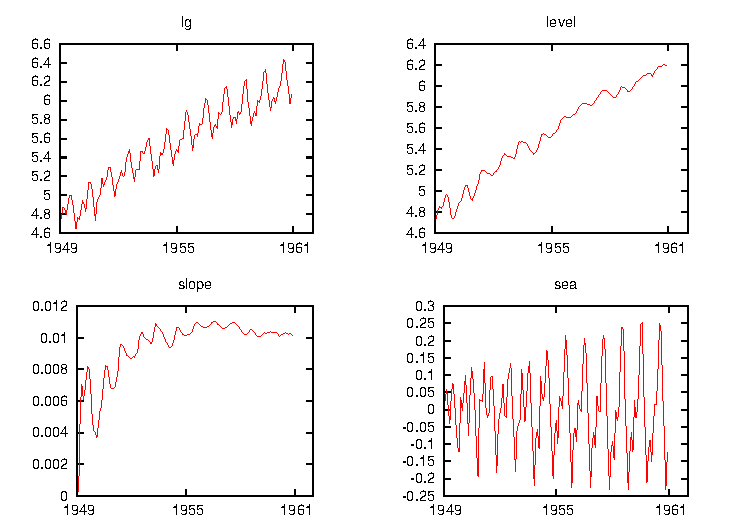
\includegraphics{figures/BSM-output}
  \caption{Estimated components from BSM}
  \label{fig:BSM-output}
\end{figure}

After the above commands have been executed, three new series will
have appeared in the gretl workspace, namely the estimates of
the three components; by plotting them together with the original
data, you should get a graph similar to
Figure~\ref{fig:BSM-output}. The estimates of the variances can be
seen by printing the \texttt{vars} matrix, as in

\begin{code}
? print vars
vars (4 x 1)

  0.00077185 
      0.0000 
   0.0013969 
      0.0000 
\end{code}

That is,
\begin{equation*}
  \hat{\sigma}^2_{\eta} = 0.00077185, \quad
  \hat{\sigma}^2_{\zeta} = 0, \quad
  \hat{\sigma}^2_{\omega} = 0.0013969, \quad
  \hat{\sigma}^2_{\varepsilon} = 0
\end{equation*}
Notice that, since $\hat{\sigma}^2_{\zeta} = 0$, the estimate for
$\beta_t$ is constant and the level component is simply a random walk
with a drift.

\section{Interacting with \app{R} from the command line}
\label{sec:foreign-command}

Up to this point we have spoken only of interaction with \app{R} via
the GUI program. In order to do the same from the command line
interface, gretl provides the \texttt{foreign} command. This
enables you to embed non-native commands within a gretl
script.

A ``foreign'' block takes the form
\begin{code}
foreign language=R [--send-data[=list]] [--quiet]
    ... R commands ...
end foreign
\end{code}
and achieves the same effect as submitting the enclosed \app{R}
commands via the GUI in the non-interactive mode (see
section~\ref{sec:R-scripts} above). The \option{send-data} option
arranges for auto-loading of the data present in the gretl session, or
a subset thereof specified via a named list.  The \option{quiet}
option prevents the output from \app{R} from being echoed in the gretl
output.

\begin{script}[htbp]
  \caption{Estimation of the Basic Structural Model -- simple}
\begin{scode}
open bjg.gdt

foreign language=R --send-data
    y <- gretldata[, "lg"]
    strmod <- StructTS(y)
    compon <- as.ts(tsSmooth(strmod))
    vars <- as.matrix(strmod$coef)
    gretl.export(compon)
    gretl.export(vars)
end foreign

append @dotdir/compon.csv
rename level lg_level
rename slope lg_slope
rename sea lg_seas

vars = mread("vars.mat", 1)
\end{scode}
\label{RStructTS-simple}
\end{script}
%$

Using this method, replicating the example in the previous subsection
is rather easy: basically, all it takes is encapsulating the content
of the \app{R} script in a \texttt{foreign}\ldots\texttt{end foreign}
block; see example \ref{RStructTS-simple}.

\begin{script}[htbp]
  \caption{Estimation of the Basic Structural Model -- via a function}
\begin{scode}
function list RStructTS(series myseries)
    smpl ok(myseries) --restrict
    sx = argname(myseries)

    foreign language=R --send-data --quiet
        @sx <- gretldata[, "myseries"]
        strmod <- StructTS(@sx)
        compon <- as.ts(tsSmooth(strmod))
        gretl.export(compon)
    end foreign

    append @dotdir/compon.csv
    rename level @sx_level
    rename slope @sx_slope
    rename sea @sx_seas

    list ret = @sx_level @sx_slope @sx_seas
    return ret
end function

# ------------ main -------------------------

open bjg.gdt
list X = RStructTS(lg)
\end{scode}

\label{RStructTS-func}
\end{script}

The above syntax, despite being already quite useful by itself, shows
its full power when it is used in conjunction with user-written
functions.  Listing~\ref{RStructTS-func} shows how to define a
gretl function that calls \app{R} internally.

\section{Performance issues with \app{R}}
\label{sec:R-performance}

\app{R} is a large and complex program, which takes an appreciable
time to initialize itself.  In interactive use this not a significant
problem, but if you have a gretl script that calls \app{R} repeatedly
the cumulated start-up costs can become bothersome.  To get around
this, gretl calls the \app{R} shared library by preference; in this
case the start-up cost is borne only once, on the first invocation of
\app{R} code from within gretl.

Support for the \app{R} shared library is built into the gretl
packages for MS Windows and OS X---but the advantage is realized
only if the library is in fact available at run time.  If you are
building gretl yourself on Linux and wish to make use of the
\app{R} library, you should ensure (a) that \app{R} has been built
with the shared library enabled (specify \verb|--enable-R-shlib| when
configuring your build of \app{R}), and (b) that the \verb|pkg-config|
program is able to detect your \app{R} installation.  We do not link
to the \app{R} library at build time, rather we open it dynamically on
demand. The gretl GUI has an item under the
\textsf{Tools/Preferences} menu which enables you to select the
path to the library, if it is not detected automatically.  

If you have the \app{R} shared library installed but want to force
gretl to call the \app{R} executable instead, you can do
\begin{code}
set R_lib off
\end{code}

\section{Further use of the \app{R} library}
\label{sec:R-functions}

Besides improving performance, as noted above, use of the \app{R}
shared library makes possible a further refinement.  That is, you can
define functions in \app{R}, within a \texttt{foreign} block, then
call those functions later in your script much as if they were
gretl functions.  This is illustrated below.  
%
\begin{code}
set R_functions on
foreign language=R
  plus_one <- function(q) {
     z = q+1
     invisible(z)
  }
end foreign

scalar b=R.plus_one(2)
\end{code}
%
The \app{R} function \verb|plus_one| is obviously trivial in itself,
but the example shows a couple of points.  First, for this mechanism
to work you need to enable \verb|R_functions| via the \texttt{set}
command.  Second, to avoid collision with the gretl function
namespace, calls to functions defined in this way must be prefixed
with ``\texttt{R.}'', as in \verb|R.plus_one|. But note, this
mechanism will not work if you have defined a gretl bundle named
\texttt{R}: in that case identifiers beginning with ``\texttt{R.{}}''
will be understood as referring to members of the bundle in question.

Built-in \app{R} functions may also be called in this way, once
\verb|R_functions| is set \texttt{on}.  For example one can invoke
\app{R}'s \texttt{choose} function, which computes binomial
coefficients:
%
\begin{code}
set R_functions on
scalar b = R.choose(10,4)
\end{code}
%
Note, however, that the possibilities for use of built-in \app{R}
functions are limited; only functions whose arguments and return
values are sufficiently generic (basically scalars, matrices or
strings) will work.

%%% Local Variables: 
%%% mode: latex
%%% TeX-master: "gretl-guide"
%%% End: 

